\documentclass[aspectratio=43,10pt]{beamer}
\usetheme{Madrid}
\usepackage{amsmath,amssymb,booktabs,tikz}
\usefonttheme{professionalfonts}
\setbeamercolor{alerted text}{parent=structure}
\newcommand{\R}{\mathbf r}
\newcommand{\V}{\mathbf v}
\newcommand{\X}{\mathbf x}
\newcommand{\dv}{\Delta\mathbf v}
\newcommand{\sr}{\mathbf s_r}
\newcommand{\sv}{\mathbf s_v}
\newcommand{\W}{\mathbf w}
\newcommand{\norm}[1]{\left\lVert #1\right\rVert}
\newcommand{\kms}{\mathrm{km/s}}
\newcommand{\km}{\mathrm{km}}
\newcommand{\lead}[1]{{\usebeamercolor[fg]{structure}\bfseries #1}}
\title[Hohmann transfer]{Hohmann Transfer via Sequential Convex Programming}
\subtitle{Two impulsive burns between circular Earth orbits}
\author[Hudson Kim]{Hudson Kim}
\institute[UC Berkeley]{University of California, Berkeley}
\date{November 2026}

\begin{document}
\begin{frame}
  \titlepage
\end{frame}

\begin{frame}{The restricted two-body equation}
Let $M$ and $m$ be the masses of Earth and the spacecraft. In an inertial frame their positions are $\mathbf R_E$ and $\mathbf R_s$. Define $\R=\mathbf R_s-\mathbf R_E$ and $r=\norm{\R}_2$.
\[
  m\ddot{\mathbf R}_s=-\frac{GMm}{r^3}\R,
  \qquad M\ddot{\mathbf R}_E=+\frac{GMm}{r^3}\R ,
\]
where $G$ is the gravitational constant. Subtract the accelerations:
\[
  \ddot{\R}=\ddot{\mathbf R}_s-\ddot{\mathbf R}_E
       =-\frac{G(M+m)}{r^3}\R .
\]
For $m\ll M$, set $\mu=GM$. Between burns, gravity alone gives
\[
  \alert{\boxed{\ddot{\R}=-\mu\R/r^3}} .
\]
\note{Treat Earth as spherical and the spacecraft as a point mass. The subtraction is exact before applying the small-mass approximation. Reference: Bryan Weber, Orbital Mechanics and Astrodynamics, Relative Motion in the Two-Body Problem.}
\end{frame}

\begin{frame}{Energy and angular momentum during the coast}
Let $\V=\dot{\R}$ and $v=\norm{\V}_2$. Dot the acceleration with velocity and use $\R\cdot\V=r\dot r$:
\[
  \frac{d}{dt}\frac{v^2}{2}
    =\V\cdot\ddot{\R}=-\mu\frac{\dot r}{r^2}
    =\frac{d}{dt}\frac{\mu}{r}.
\]
Thus the \lead{specific orbital energy} is constant:
\[
  \varepsilon=\frac{v^2}{2}-\frac{\mu}{r}.
\]
Gravity also exerts zero torque about Earth. The \lead{specific angular momentum} $\mathbf h=\R\times\V$ satisfies
\[
  \dot{\mathbf h}=\V\times\V+\R\times\ddot{\R}=\mathbf 0.
\]
\note{Specific means per unit spacecraft mass. Both conserved quantities apply on each unpowered arc. Reference: Bryan Weber, Orbital Mechanics and Astrodynamics, Energy Is Conserved in Orbital Motion.}
\end{frame}

\begin{frame}{Vis-viva from the two apsides}
Let $r_p<r_a$ be periapsis and apoapsis on an ellipse, with speeds $v_p,v_a$. At each apsis $\R\perp\V$, so $H=\norm{\mathbf h}_2=r_pv_p=r_av_a$.
\[
  \frac{H^2}{2r_p^2}-\frac{\mu}{r_p}
  =\frac{H^2}{2r_a^2}-\frac{\mu}{r_a}
  \quad\Longrightarrow\quad H^2=\frac{2\mu r_pr_a}{r_p+r_a}.
\]
Substitution at periapsis gives the energy in terms of the semimajor axis $a=(r_p+r_a)/2$:
\[
  \varepsilon=\frac{\mu r_a}{r_p(r_p+r_a)}-\frac{\mu}{r_p}
    =-\frac{\mu}{r_p+r_a}=-\frac{\mu}{2a}.
\]
At any radius on the ellipse, $v^2/2-\mu/r=-\mu/(2a)$. Hence
\[
  \alert{\boxed{v^2=\mu\!\left(\frac{2}{r}-\frac1a\right)}} .
  \qquad \text{Circular limit }(a=r):\quad v_c(r)=\sqrt{\mu/r}.
\]
\note{At the two apsides the radial velocity vanishes. Using angular momentum first removes the two unknown speeds from the energy balance. The circle follows by continuity.}
\end{frame}

\begin{frame}{Geometry of the transfer ellipse}
\begin{columns}[onlytextwidth,c]
\begin{column}{.49\textwidth}
The spacecraft leaves the inner circle at periapsis, at radius $r_1$. It reaches the outer circle at apoapsis, at radius $r_2$.
\medskip

Earth is at a focus of the ellipse. The distance between the two burn points is its major axis:
\[
  2a_t=r_1+r_2.
\]
\end{column}
\begin{column}{.49\textwidth}
\centering
% Scale the outer circular radius to 2.35. Earth is at the lower focus.
\begin{tikzpicture}[x=1cm,y=1cm]
  \pgfmathsetmacro{\ro}{2.35}
  \pgfmathsetmacro{\ri}{\ro*6.569487/42.159137}
  \pgfmathsetmacro{\majoraxis}{(\ri+\ro)/2}
  \pgfmathsetmacro{\minoraxis}{sqrt(\ri*\ro)}
  \pgfmathsetmacro{\centerheight}{(\ro-\ri)/2}
  \draw[black!45,thin] (0,0) circle (\ro);
  \fill[blue!15] (0,0) circle ({\ri*6.378137/6.569487});
  \draw[black!50,thin] (0,0) circle (\ri);
  \draw[structure.fg,very thick] plot[domain=-90:90,samples=90]
    ({\minoraxis*cos(\x)},{\centerheight+\majoraxis*sin(\x)});
  \fill[structure.fg] (0,-\ri) circle (1.8pt) (0,\ro) circle (1.8pt);
  \node[below right,inner sep=2pt,font=\scriptsize] at (0,-\ri) {Departure};
  \node[above,font=\scriptsize] at (0,\ro) {Arrival};
\end{tikzpicture}
\end{column}
\end{columns}
\end{frame}

\begin{frame}{The analytical Hohmann transfer}
The transfer ellipse touches the departure circle at $r_1$ and the arrival circle at $r_2$. Here $a_t=(r_1+r_2)/2$ and $r_2>r_1$.
\[
\begin{aligned}
\Delta v_{H,1}
 &=\sqrt{\mu\!\left(\frac{2}{r_1}-\frac1{a_t}\right)}
      -\sqrt{\frac{\mu}{r_1}}
  &&\text{enter the ellipse},\\[4pt]
\Delta v_{H,2}
 &=\sqrt{\frac{\mu}{r_2}}
      -\sqrt{\mu\!\left(\frac{2}{r_2}-\frac1{a_t}\right)}
  &&\text{circularize}.
\end{aligned}
\]
Both impulses are prograde. The coast covers half an orbital period:
\[
 \Delta v_H=\Delta v_{H,1}+\Delta v_{H,2},
 \qquad t_H=\pi\sqrt{a_t^3/\mu}.
\]
\end{frame}

\begin{frame}{Numerical benchmark}
With Earth's radius $R_E=6378.137\ \km$ and $\mu=398600.44\ \mathrm{km^3/s^2}$, the reference case is
\begin{center}
\begin{tabular}{lrr}
\toprule
 & Departure & Arrival\\ \midrule
Altitude (km) & $191.35$ & $35{,}781$\\
Radius (km) & $6{,}569.487$ & $42{,}159.137$\\
Burn magnitude (km/s) & $2.457$ & $1.478$\\ \bottomrule
\end{tabular}
\end{center}
\[
 \alert{\Delta v_H=3.935\ \kms}
 \qquad\qquad
 \alert{t_H=5.26\ \mathrm{h}}
\]
The optimization fixes the coast time at $t_H$ and solves for both burn vectors.
\end{frame}

\begin{frame}{Planar states and endpoint conditions}
At each of $N$ nodes, let $\X_k=(\R_k,\V_k)$ with $\R_k=(x_k,y_k)$ in km and $\V_k=(v_{x,k},v_{y,k})$ in km/s. Pairs denote column vectors.
\medskip

\lead{Departure.} Node $0$ is immediately after the first burn.
\[
  \R_0=(0,-r_1), \qquad \V_0=(\sqrt{\mu/r_1},0)+\dv_1 .
\]
\lead{Arrival.} Node $N-1$ is immediately before the second burn.
\[
\begin{aligned}
  \R_{N-1} &= (0,r_2)+\sr ,\\
  \V_{N-1}+\dv_2 &= (-\sqrt{\mu/r_2},0)+\sv .
\end{aligned}
\]
The signed terminal errors $\sr$ (km) and $\sv$ (km/s) vanish for an exact transfer. Each impulse changes only velocity.
\end{frame}

\begin{frame}{Linearizing the coast dynamics}
For the planar state $\X=(x,y,v_x,v_y)^T$, let $r=\sqrt{x^2+y^2}$. The nonlinear state derivative is
\[
  \dot{\X}=f(\X)=
   \begin{bmatrix}v_x & v_y & -\mu x/r^3 & -\mu y/r^3\end{bmatrix}^{T}.
\]
At node $k$, fix a reference state $\bar\X_k$ and take the first-order Taylor expansion:
\[
  A_k=\left.\frac{\partial f}{\partial\X}\right|_{\bar\X_k},\qquad
  \alert{f_{\mathrm{lin},k}(\X_k)=f(\bar\X_k)+A_k(\X_k-\bar\X_k)} .
\]
Within one solve, $f(\bar\X_k)$ and $A_k$ are fixed. The new state $\X_k$ enters the dynamics affinely.
\end{frame}

\begin{frame}{The gravity Jacobian}
Write $\bar\R=(\bar x,\bar y)^T$ and $\bar r=\norm{\bar\R}_2$ at node $k$. Differentiating $-\mu\R/r^3$ with respect to position gives
\[
  \frac{\partial\ddot{\R}}{\partial\R}
  =\frac{3\mu}{\bar r^5}\bar\R\bar\R^T-\frac{\mu}{\bar r^3}I_2 .
\]
The full state Jacobian, ordered as $(x,y,v_x,v_y)$, is
\[
 A_k=\begin{bmatrix}
 0 & 0 & 1 & 0\\
 0 & 0 & 0 & 1\\[2pt]
 \dfrac{3\mu\bar x^2}{\bar r^5}-\dfrac{\mu}{\bar r^3} &
 \dfrac{3\mu\bar x\bar y}{\bar r^5} & 0 & 0\\[7pt]
 \dfrac{3\mu\bar x\bar y}{\bar r^5} &
 \dfrac{3\mu\bar y^2}{\bar r^5}-\dfrac{\mu}{\bar r^3} & 0 & 0
 \end{bmatrix}.
\]
\note{The upper right identity comes from the kinematic relation between position and velocity. Gravity has no velocity dependence, so the lower right block is zero.}
\end{frame}

\begin{frame}{Two discretizations of the same coast}
Set $h=t_H/(N-1)$ and $t_k=kh$. The exact update integrates the state derivative:
\[
 \X_{k+1}=\X_k+\int_{t_k}^{t_{k+1}} f(\X(t))\,dt .
\]
For each interval let $F_k=f_{\mathrm{lin},k}(\X_k)$ and let $\W_k\in\mathbb R^4$ be a dynamics slack.
\begin{align*}
 \text{Forward Euler}\qquad &\X_{k+1}=\X_k+h F_k+\W_k,\\[5pt]
 \text{Trapezoidal}\qquad &\X_{k+1}=\X_k+\tfrac h2(F_k+F_{k+1})+\W_k .
\end{align*}
The trapezoidal step uses a separate linearization at $\bar\X_{k+1}$. Both constraints are affine. For smooth dynamics with zero slack, the integration rules have global orders $O(h)$ and $O(h^2)$, respectively.
\end{frame}

\begin{frame}{The convex subproblem}
Choose the states $\{\X_k\}$, impulses $\dv_1,\dv_2\in\mathbb R^2$, interval slacks $\{\W_k\}$, and terminal slacks $\sr,\sv\in\mathbb R^2$. Minimize
\[
 \underbrace{\norm{\dv_1}_2+\norm{\dv_2}_2}_{\text{total burn magnitude}}
 +\underbrace{\lambda_d\sum_{k=0}^{N-2}\norm{\W_k}_1
 +\lambda_r\norm{\sr}_1+\lambda_v\norm{\sv}_1}_{\text{penalties on dynamics and endpoint errors}} .
\]
Enforce the endpoint conditions and one discretized dynamics constraint per interval. At every node, bound each component of the state update:
\[
 \norm{\R_k-\bar\R_k}_\infty\leq\rho_r=100\ \km,\qquad
 \norm{\V_k-\bar\V_k}_\infty\leq\rho_v=0.5\ \kms .
\]
The positive weights $\lambda_d,\lambda_r,\lambda_v$ set the cost of each slack. The implementation uses $10^3$ for all three with states in km and km/s.
\end{frame}

\begin{frame}{The first reference trajectory}
Start with a trial tangential speed and propagate the nonlinear coast. The write-up tests speeds such as $1.25\,v_c(r_1)$ and $1.30\,v_c(r_1)$.
\medskip

Let $\R_\star=(0,r_2)$ be the target. An exact terminal position and the endpoint trust region can hold together only if
\[
   \norm{\R_\star-\bar\R_{N-1}}_\infty\leq 100\ \km .
\]
A reference endpoint thousands of kilometers away violates this condition. Allowing $\R_{N-1}=\R_\star+\sr$ lets the first solve take a bounded step toward the target.
\medskip

After each solve, replace $\bar\X_k$ with the new $\X_k$ and linearize again. The trust region moves with the reference.
\end{frame}

\begin{frame}{A separate check on arrival accuracy}
A small change between SCP iterates can coexist with nonzero slacks or integration error. First inspect $\W_k$, $\sr$, and $\sv$.
\medskip

Then apply the optimized departure impulse and integrate the original two-body equations for $t_H$. The visualizer uses fourth-order Runge--Kutta with steps of at most 10 s. Let $\R_{\rm prop},\V_{\rm prop}$ denote that coast.
\[
\begin{aligned}
 e_r&=\norm{\R_{\rm prop}(t_H)-(0,r_2)}_2,\\[3pt]
 e_v&=\norm{\V_{\rm prop}(t_H)+\dv_2-(-\sqrt{\mu/r_2},0)}_2 .
\end{aligned}
\]
The reported \lead{arrival miss} is $e_r$. An instantaneous second burn can change $e_v$ but cannot correct an existing position error at $t_H$.
\end{frame}

\begin{frame}{Forward Euler misses the target by 21,585.7 km}
\centering
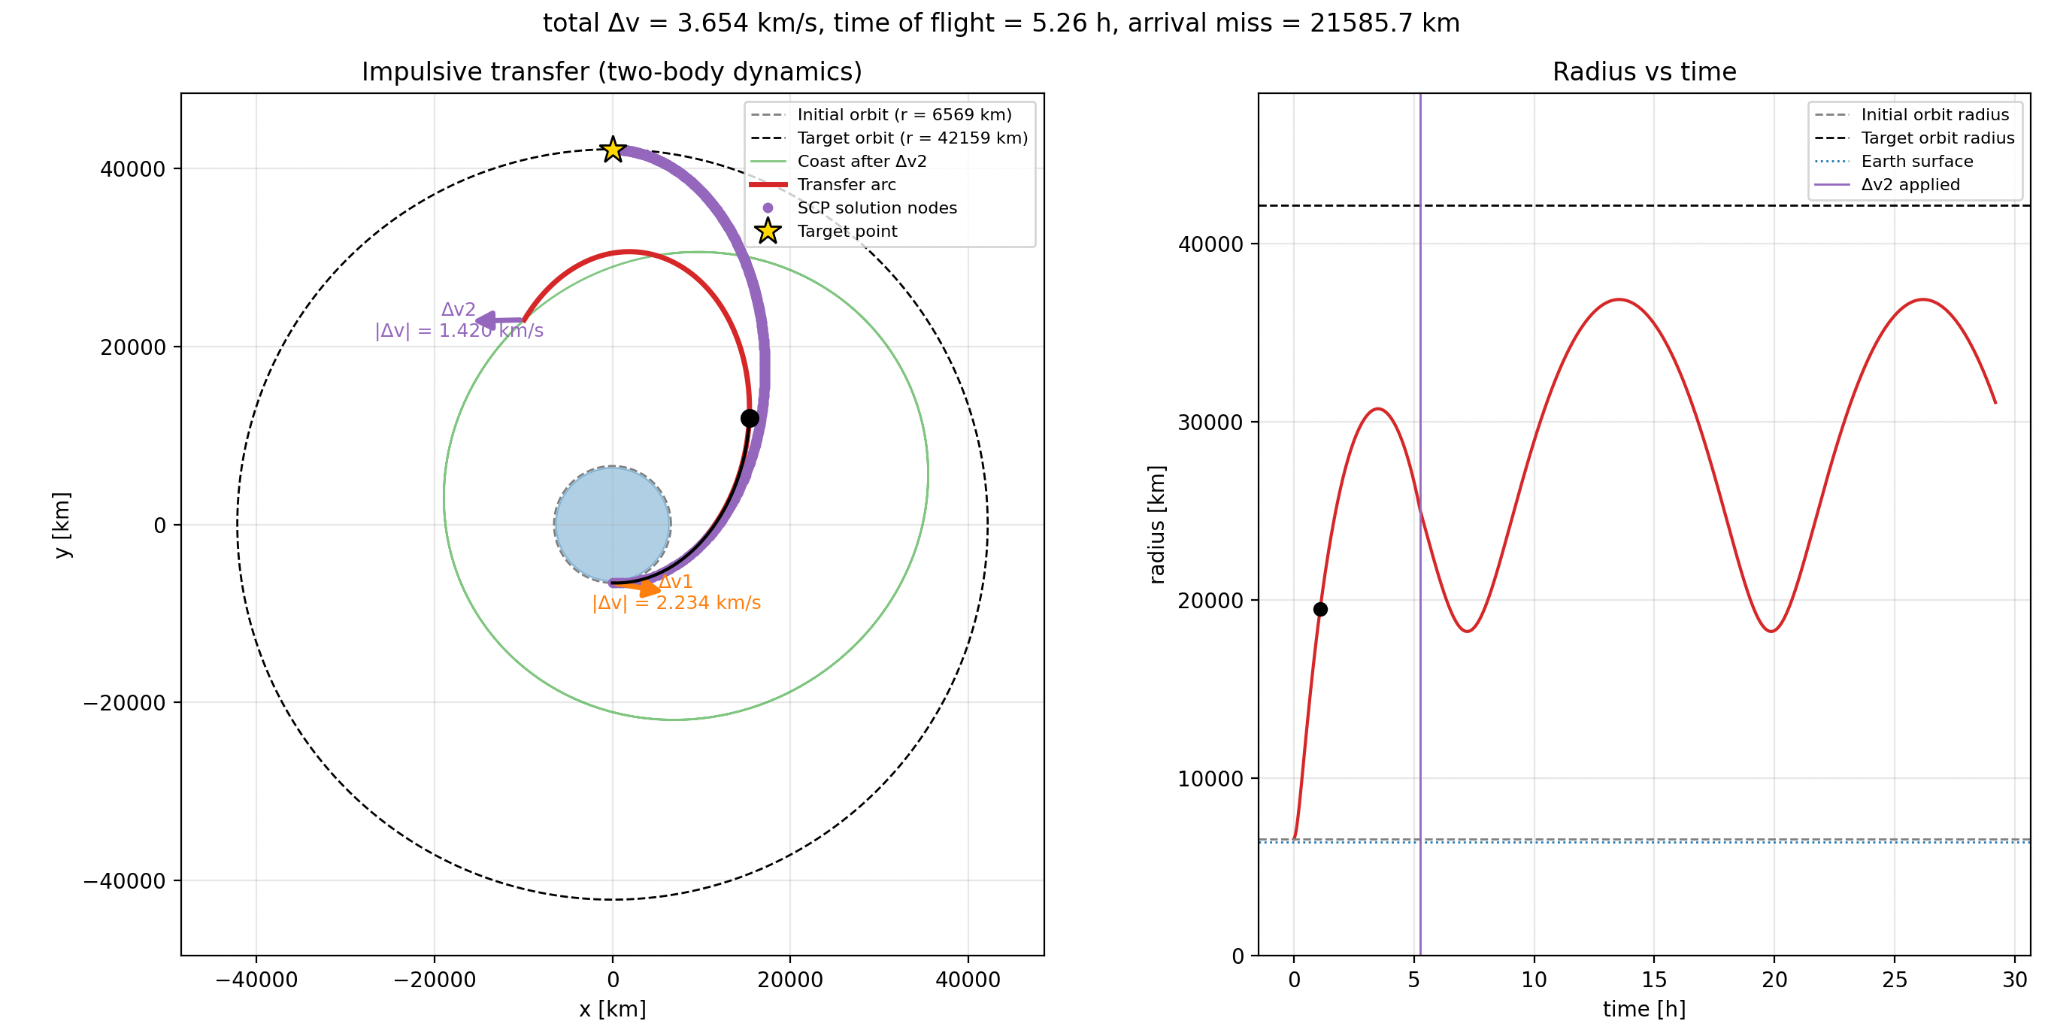
\includegraphics[width=\textwidth,height=.69\textheight,keepaspectratio]{figures/forward_euler_updated.png}\par
\smallskip
The red nonlinear coast separates from the purple SCP nodes before arrival.
\end{frame}

\begin{frame}{The trapezoidal solution misses by 205.7 km}
\centering
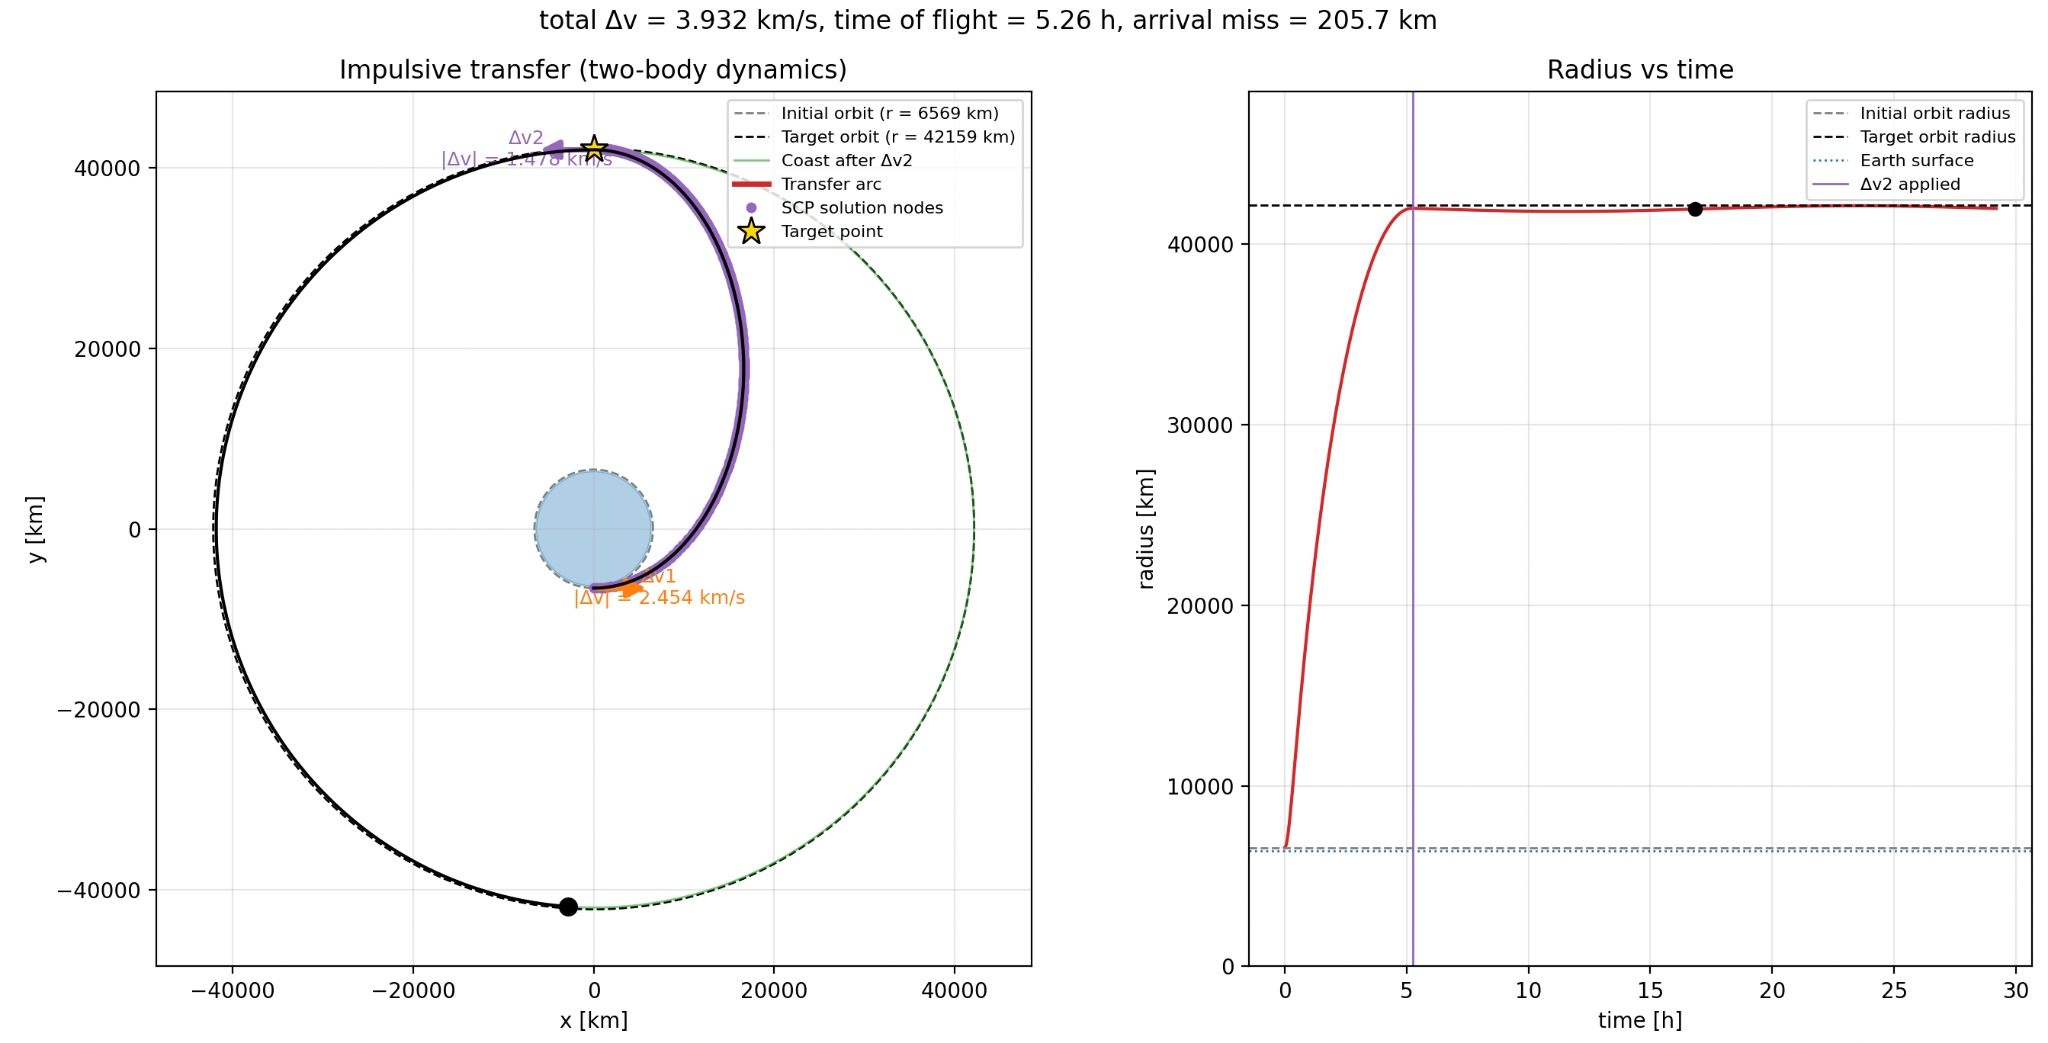
\includegraphics[width=\textwidth,height=.69\textheight,keepaspectratio]{figures/trapezoidal_updated.png}\par
\smallskip
The propagated transfer tracks the nodes closely at the scale of the orbit.
\end{frame}

\begin{frame}{Burn cost and arrival accuracy}
Both numerical solutions use the same departure and arrival orbits and the same Hohmann coast time.
\begin{center}
\renewcommand{\arraystretch}{1.26}
\begin{tabular}{lrr}
\toprule
Method & Total $\Delta v$ (km/s) & Arrival miss (km)\\
\midrule
Analytical Hohmann & $3.935$ & $\approx 0$\\
Forward Euler & $3.654$ & $21{,}585.7$\\
Trapezoidal & $3.932$ & $205.7$\\
\bottomrule
\end{tabular}
\end{center}
Forward Euler's lower burn cost accompanies a large endpoint error. The trapezoidal result comes within about \lead{3 m/s} of the analytical cost, but the propagated spacecraft still arrives \lead{205.7 km} from the target.
\end{frame}
\end{document}
